% !TeX root = main.tex

% ============================================================
% thesis-sync entry: 2026-07-19_inchworm-performance-gaits
% Type: experimental result (forward / steering / transition gaits)
% Part of the INCHWORM ROBOT block (prior work, precedes the lizard sections).
% Insertable section block (no preamble). Requires: graphicx.
% ============================================================

\section{LOCOMOTION PERFORMANCE}
\label{sec:inchworm-performance}

The locomotion performance of the proposed soft robot was evaluated on a
substrate inclined at $60^\circ$ relative to the horizontal.

\subsection{Forward Gait}

The fundamental forward locomotion sequence (Fig.~\ref{fig:inchworm-performance},
row~1) consists of four distinct phases. The cycle initiates (Phase~1) from
an unpressurized, linear configuration, with the anterior suction cup engaged
to anchor the system to the substrate. During Phase~2, a small positive
pressure is applied to disengage the posterior suction cup, and the superior
internal chamber is pressurized; this induces a bending deformation in the
actuator, drawing the posterior extremity forward. In Phase~3, the anchorage
is reversed: the anterior cup is disengaged to permit sliding, while the
posterior cup is engaged to secure the robot. Finally, in Phase~4, all three
internal chambers are simultaneously pressurized to drive longitudinal
extension; this straightens the actuator, advances the anterior suction cup,
and resets the robot for the subsequent cycle.

\subsection{Steering Gait}

The steering gait (Fig.~\ref{fig:inchworm-performance}, row~2) cycle diverges
from the forward trajectory exclusively during Phase~2. To achieve
directional change, the superior chamber is pressurized concurrently with one
of the lateral chambers. This asymmetric inflation induces an off-axis
spatial bend, resulting in a net $16^\circ$ directional turn upon the
completion of Phase~4.

\subsection{Floor-to-Wall Transition Gait}

The floor-to-wall transition gait (Fig.~\ref{fig:inchworm-performance},
rows~3--4) consists of a 15-step sequence designed to cross the boundary
between a horizontal and an inclined surface. To initiate this maneuver,
pressurizing one of the lateral chambers bends the actuator sideways, guiding
the disengaged anterior suction cup around the edge. Subsequently, inflating
both lateral chambers simultaneously bends the actuator upward, lifting the
cup over the edge to reach and anchor onto the incline. Once secured, the
remaining steps follow the standard forward gait sequence to advance the
posterior segment of the robot onto the wall.

\subsection{Summary}

This chapter presented a novel soft inchworm climbing robot designed to
overcome the limitations of planar locomotion by enabling omnidirectional
maneuverability and complex surface transitions. Driven by a single
fiber-reinforced, three-chambered pneumatic actuator, the robot uniquely
couples both bending and longitudinal elongation within its fundamental gait.
This approach differentiates the robot from traditional inchworm
architectures and facilitates versatile 3D mobility. To maximize efficiency,
the actuator's structural parameters were optimized via FEM to significantly
reduce the pressure required for bending. Concurrently, a custom
multi-channel pneumatic system enabled independent, closed-loop pressure
control, governed by a discrete-time SMC algorithm to ensure robust,
chatter-free regulation. Kinematic testing on a $60^\circ$ incline confirmed
the efficacy of the design, validating its ability to execute a forward gait,
asymmetric steering, and a complete floor-to-wall transition sequence. The
three-chambered omnidirectional actuator and multichannel pneumatic control
established here form the foundation for the lizard-inspired soft robot
developed in the subsequent chapters.

\begin{figure*}[tb]
  \centering
  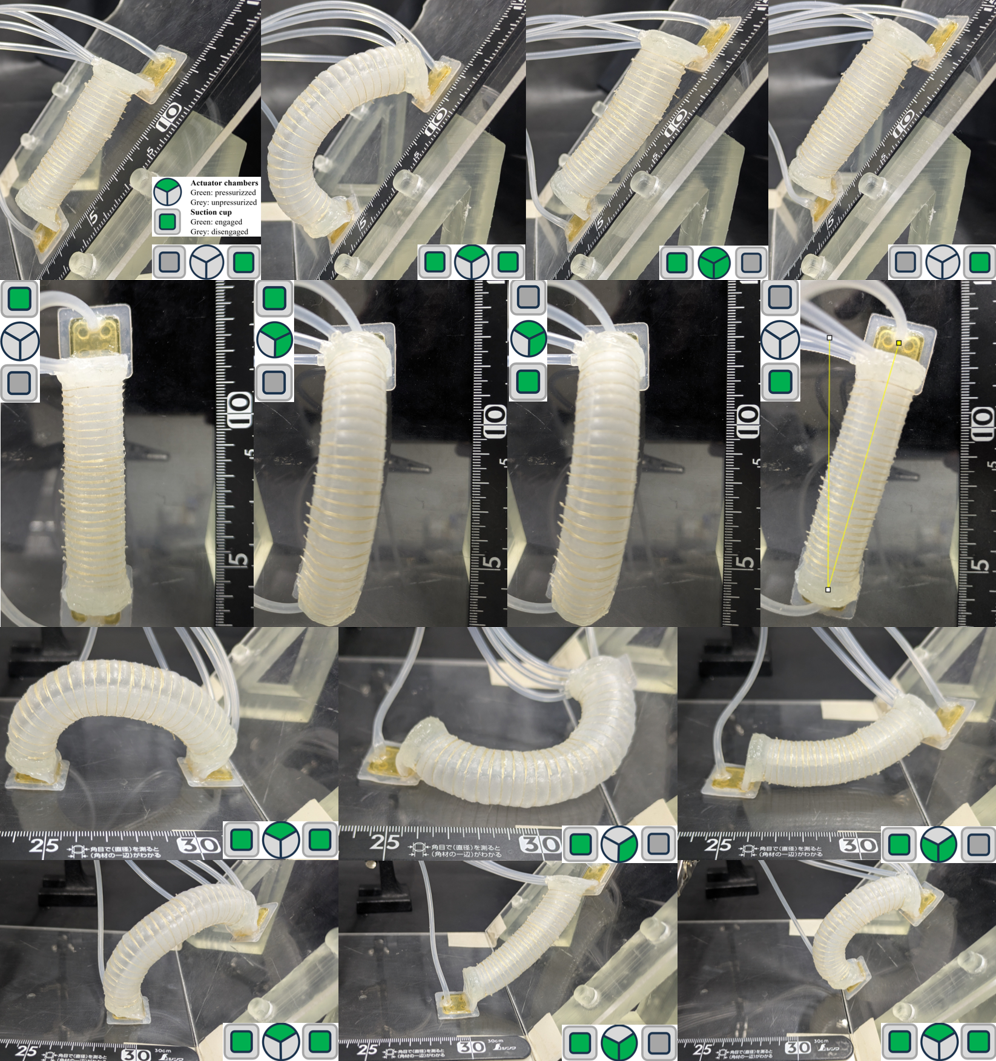
\includegraphics[height=165mm]{figures/performance.eps}
  \vspace*{-2mm}
  \caption{Soft robot performance on a $60^\circ$ incline. (Row~1) Forward
  gait. (Row~2) Steering gait. (Rows~3--4) Floor-to-wall transition gait.}
  \label{fig:inchworm-performance}
\end{figure*}
